\clearpage
\section{Slipring}

To allow the laser sensor to continuously rotate and take measurements, a slip ring is needed to avoid issues with the cables breaking or getting tangled. This results in damage to the equipment. 
The slip ring used for this build is a SNM022A-06\cite{slipring}, which is a 6-wire slip ring that supports up to 210DC/240AC. 

\begin{figure}[H]
	\centering
	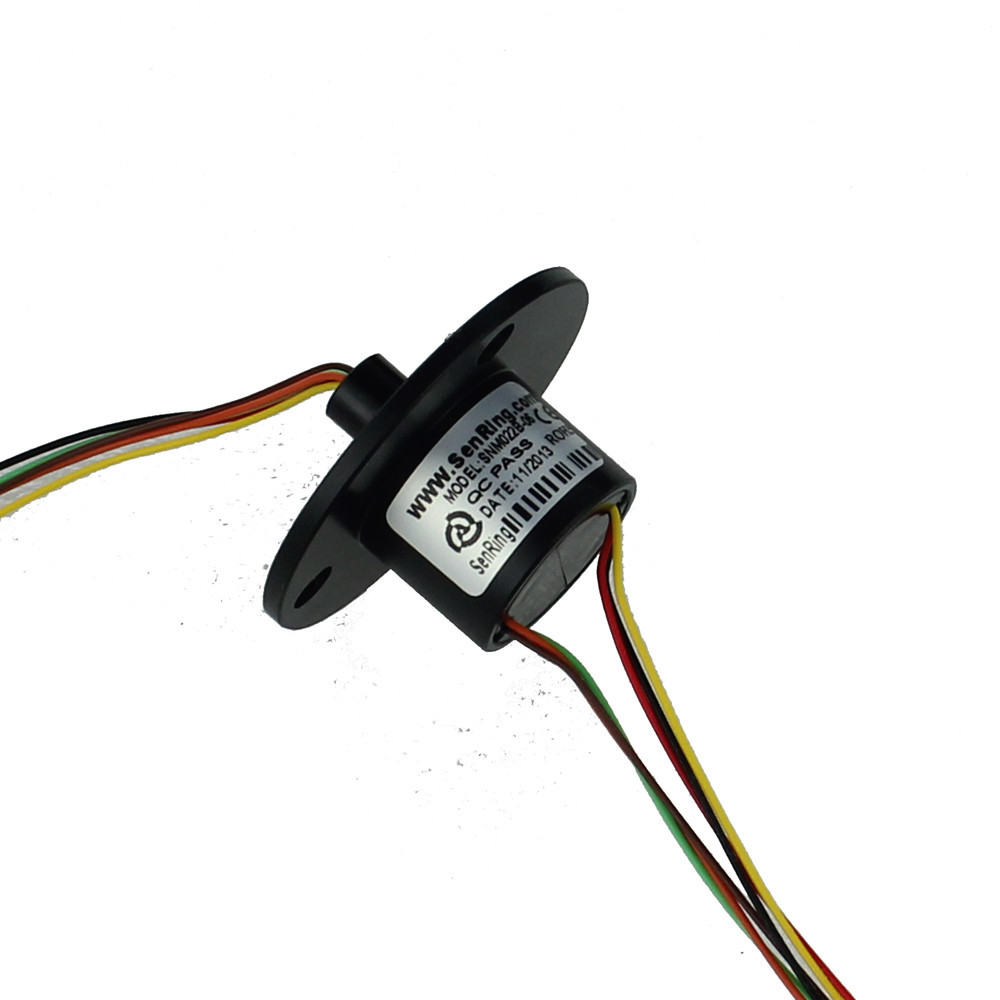
\includegraphics[width=.5\linewidth]{images/slipring-pic.jpg}
	\caption{The SNM022A-06}
	\label{slipringpic}	
\end{figure}

The slip ring allows the transfer of electrical signal from a stationary object to a rotating object. The center of the slip ring remains stationary as the surrounding housing rotates, in our case 6, conducting brushes along the center core in separate lanes, which then transfers the electrical signal.
The specific slip ring used has 6 lanes on the core, since the slip ring is compatible up to 6 wires. Between each of the lanes a high resistance insulation is put into place to avoid short circuits and signal interference between the wires.\cite{slipringhow} \\
Slip rings are often used in electrical generators, in cable reels and wind turbines.


